%          spconf.sty  - ICASSP/ICIP LaTeX style file, and
%          IEEEbib.bst - IEEE bibliography style file.
% --------------------------------------------------------------------------
\documentclass{article}
\usepackage{spconf,amsmath,graphicx}
\usepackage{booktabs}
\usepackage{hyperref}
\usepackage{float}
\usepackage{amssymb}
\usepackage{caption}
\usepackage{subcaption}

\usepackage[backend=bibtex,style=numeric,sorting=none]{biblatex}
\addbibresource{refs.bib}
\renewcommand*{\bibfont}{\footnotesize}

\usepackage[toc,page]{appendix}


\setlength\parindent{0pt}

\graphicspath{ {img/} }

% Title.
% ------
\title{Applied machine learning system ELEC0134 20/21 report}
\name{SN: 17011729}
\address{}
%
\begin{document}
%
\maketitle
%
\begin{abstract}
    Four different classification tasks were performed on two distinct datasets. Both datasets have facial images as data samples but one is of humans while the other is of cartoons. On human faces, gender detection and smile detection problems were tackled while multi-class face-shape and eye-colour classification was tackled on the cartoon faces. The selection of models, pre-processing of images as well as hyper-parameter tuning techniques are discussed. A convolutional neural network was used for the gender classification while facial landmarks around the mouth were extracted as features to be trained by an SVM for smile detection. These models resulted in accuracies of 91.1\% and 84.5\% respectively. An SVM was used for the face-shape classification as well (99.0\%) while a random forest was utilized for the eye-colour classification (83.0\%).
    
    \href{https://github.com/tharmee99/AMLS_assignment20_21}{Link to GitHub Repository}\footnote{https://github.com/tharmee99/AMLS\_assignment20\_21}
\end{abstract}
%
\begin{keywords}
    Convolutional Neural Network, Facial Detection, Support Vector Machine, Random Forests, Feature Extraction, Classification
\end{keywords}
%

\section{Introduction}
\label{sec:introduction}
    Machine learning has been increasingly used to solve classification and regression tasks for which traditional algorithms either don't exists or perform poorly in comparison. Facial detection and classification is a common problem tackled by Machine Learning techniques. Techniques discussed by Viola and Jones \autocite{990517} have been widely used and were a large stepping stone to more complex facial detection/classification algorithms \autocite{8806572, 8549735}. Furthermore, the introduction of convolutional neural networks (CNNs) transformed feature extraction and classification in image datasets even more \autocite{6619290, 7553523}.
    \\
    
    This project aims to solve 4 classification tasks on 2 different datasets. The datasets being used are a subset of the "Cartoon Set" (cartoonset) dataset provided by Google \autocite{cartoonset} as well as a subset of the "CelebFaces Attributes" (celebA) provided by Shuo Yang et al \autocite{7410776}. While both datasets consist of image data samples, the former contains computer generated graphics of cartoon images whereas the latter contains cropped and pose corrected images of people. The celebA dataset will contain a larger variation in subject background, lighting and face position compared to the uniform nature of the cartoonset dataset. This will undoubtedly make the classification task more difficult.
    \\
    
    On the celebA dataset two binary classification tasks will be tackled; one will try to distinguish between the gender of the person (task A1) and the other will be making classifications on the emotion of the person by making decisions on whether or not they're smiling (task A2). On the cartoon dataset, two multi-class classification tasks will be considered. The first task will try to classify the face-shape of the cartoon (task B1). The final task will classify the eye-colour of the cartoon face (task B2). Face-shapes eye-colour were both limited to 5 classes each in the subset. 
    \\
    
    \S \ref{sec:literature_survey} will discuss existing architectures for facial feature extraction as well as classification and discuss their effectiveness relative to one another. \S \ref{sec:description_of_models} and \S \ref{sec:implementation_of_models} will discuss the description and implementation of the chosen models. Justification for the chosen approach will be given as well as a detailed insight into how those models were realised, trained and tested in python. The obtained results will be analysed in \S \ref{sec:experimental_results} and finally a conclusion will be drawn in \S \ref{sec:conclusion}.

\section{Literature survey}
\label{sec:literature_survey}
    Facial detection and classification in human face images is a common task tackled my machine learning and a variety of approaches exist for a multitude of different classification tasks. As previously discussed our aim in the celebA dataset is to classify gender and smiles. The approach discussed in \autocite{5170659} segments the face into 7 regions and then trains a support vector machine (SVM) on each of the segments individually. It was found that the upper region of the face as well as a single eye contained enough information on their own to classify gender with an classification rate of above 90\%. SVMs are a type of model that can be adapted to both classification and regression problems. The training of the model is a convex optimization problem suggesting that the trained model will be globally optimal \autocite{bishop_2006}. Another approach to gender classification is discussed in \autocite{6391660}. In this approach faces are localized by using haar cascade filters (similar to the approach discussed in \autocite{990517}). Following this, a number of geometric features are computed from landmarks on the detected face. These are then fed into SVM classifiers for gender classification. Another very popular method of facial feature extraction is by extracting common landmarks from the face. A common method of achieving this is an ensemble of regression trees \autocite{6909637} and are implemented in dlib \autocite{dlib_shape}. A particularly interesting discussion is provided in \autocite{7789587}. This paper discusses gender and smile classification on human face images which is the same problem that we are tackling in this project. The taken approach is to use a deep CNN to classify the different attributes. Different cropping and pre-processing steps are discussed and the model discussed is also trained on the celebA dataset. 
    \\
    
    Cartoon face classification is a less popular subject of discussion when it comes to machine learning. However, there still exist some approaches to classify different attributes of cartoon face images. Cartoon face detection using feature extraction is discussed in \autocite{takayama_2012}. An approach to segment the skin of the character using a range of HSV colours followed by a flood-fill approach of selecting the correct patch of skin. In addition to this, the jaw is identified and fitted using a quadratic equation. This approach is analogous to the face-shape classification we are posed with in this project. The jaw-fit coefficients could potentially be used as features to train a model. A face detection and recognition approach as well as dataset is provided in \autocite{1907_13394}. The approach for face detection and recognition involves state of the art deep neural network (DNN) architectures such as SphereFace \autocite{8100196} and ArcFace \autocite{8953658}. The problem discussed in this paper however is different from our scenario as the images are taken from cartoons resulting in varying pose, lighting and artistic style. On the contrary, in our problem the dataset is extremely uniform and is of identical artistic style.


\section{Description of models}
\label{sec:description_of_models}
    \subsection{Task A1: Gender Classification (Binary)}
    \label{sec:desc_A1}
    
	    This problem involves the classification of human face images into two classes: Male and Female. The images provided were pose corrected and centred requiring minimal pre-processing which is further discussed in \S \ref{sec:implement_A1}. The chosen model is a CNN with the layer configuration shown in Fig. \ref{fig:a1_cnn}. The mathematical forms of the activation functions (rectified linear unit(ReLU) and soft-max) used in the models are given below in Eq. \ref{eq:activation_functions}:
	    
	    \begin{equation}
	    	\label{eq:activation_functions}
	    	\begin{split}
	    		f_{ReLU}(\boldsymbol{z})_i &= \max(0,z_i) \;\; \text{for} \;\;  i = 1, 2, \dots , K\\
	    		f_{softmax}(\boldsymbol{z})_i &= \frac{e^{z_i}}{\sum_{j=1}^{K}e^{z_j}} \;\; \text{for} \;\;  i = 1, 2, \dots , K
	    	\end{split}
	    \end{equation}
	    
	    where $\boldsymbol{z} \in \mathbb{R}^K$ is the output of the layer.
	    \\
	    
	    \begin{figure}[htb]
	    	\centering
	    	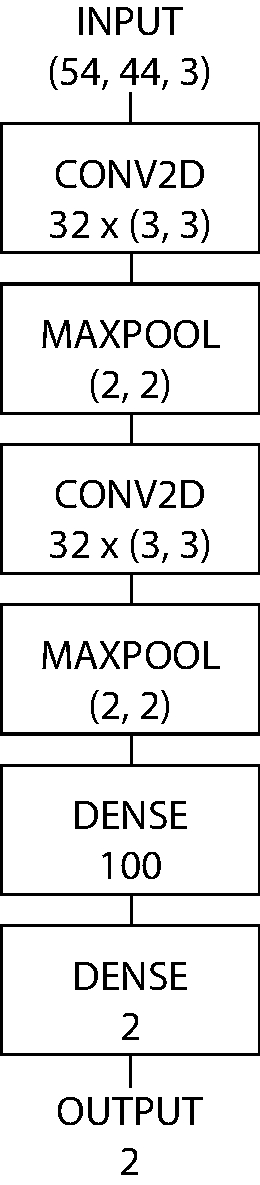
\includegraphics[scale=0.5]{a1_cnn.pdf}
	    	\caption{The layer configurations used in the model for gender classification. The layer activations for the convolutional layers as well as the penultimate dense layer are the rectified linear Unit (ReLU) for which the mathematical form is given in Eq \ref{eq:activation_functions}}
	    	\label{fig:a1_cnn}	
	    \end{figure}
	
		CNNs are commonly used with image datasets to solve classification as well as regression problems. A convolutional layer consists of multiple filters that are used to cross-correlate with the image. By doing so the filters are able to extract edges and other such simple features. The type of feature that is extracted is dependant on the filter parameters that are learnt. Deep CNNs are able to extract more complex features such as eyes, hair, mouth etc. However in this case such a deep network was not necessary to obtain reasonable results. The two Convolutional layers act to extract features from the image that correlate highly with the output labels while the max pool layers downsample the convolutional layer outputs. In this particular case, the max pool layer split the output of the convolutional layers into 2x2 sections and choose the maximum value. The resulting features and filter outputs will be discussed in further detail in \S \ref{sec:implement_A1}. The final 100 neuron dense layer will essentially "summarize" the features obtained for the 2 neuron soft-max layer. The soft-max layer will produce an output that is analogous to the one-hot encoded label meaning that the performance of the model can be computed directly by comparing the two. All hyper-parameters were tunes by using cross-validation techniques for scoring of the model. When choosing a model for this task, other models were also considered (SVM, decision trees) but neither had a good balance of accuracy and training time. The SVM was able to perform reasonable well but took incredibly long to train while the decision tree classifier easily over-fit on the data and was not able to reach reasonable accuracies.
    
    \subsection{Task A2: Emotion Classification (Binary)}
    \label{sec:desc_A2}
    
    	This task involves the classification of the emotion of the person in the image. In this case, the emotion is interpreted from the smile of the person. The labels are simply smiling and not smiling making this once again a binary classification problem. For this problem the primary feature of interest is the mouth of the person in the image. Therefore normalized landmark coordinates of the mouth were extracted as features for this task. More detail on how this was achieved will be discussed in \ref{sec:implement_A2}.
    	\\
    	
    	The chosen model for this classification task was an SVM. This was chosen as it is a relatively simple model compared to neural networks that are commonly used for image classification. In addition to this, the fact that SVMs converge to a global optimum is also beneficial when training the model. One of the biggest advantage of an SVM is the ability to use non-linear kernels. This enables the classifier to capture complex relationships without having to perform complex transformation on the data. Furthermore, the non-linear SVM provided a 2\% - 3\% increase in average test accuracy during k-fold cross validation (CV) with 5 folds compared to a K nearest neighbour classifier as well as a logistic classifier. This increase in accuracy came at no apparat change in training/testing times due to small dimension of the extracted features.
    	\\
    	
    	SVMs function by finding the maximum-margin hyperplane in an implicit high-dimensional feature space. The model doesn't compute the data points in the higher dimensional space but rather computes inner products of the lower dimensional vectors. This is achieved by utilizing the kernel trick which can be summarized as follows:
    	
    	\begin{equation}
    		\kappa\left(\boldsymbol{x}, \boldsymbol{y}\right) = \varphi\left(\boldsymbol{x}\right)^T\varphi\left(\boldsymbol{y}\right)
    	\end{equation}
    	
    	where $\varphi$ is a feature map from the low dimensional space to the higher dimensional space and $\kappa\left(\boldsymbol{x}, \boldsymbol{y}\right)$ is a function of the lower dimensional vectors. Some commonly used kernel with SVMs are the polynomial kernel and radial basis function (RBF) kernel, both of which are shown in Eq. \ref{eq:kernel_functions} below:
    	
    	\begin{equation}
    		\label{eq:kernel_functions}
    		\begin{split}
    			\kappa_{poly}\left(\boldsymbol{x}, \boldsymbol{y}\right) &= \left(1 + \boldsymbol{x^{T}}\boldsymbol{y}\right)^d \\
    			\kappa_{rbf}\left(\boldsymbol{x}, \boldsymbol{y}\right) &= \exp\left(-\gamma\left\lVert\boldsymbol{x}-\boldsymbol{y}1\right\rVert^2\right)
    		\end{split}
    	\end{equation}
    
    	where $d$ is the degree of the polynomial kernel chosen and $\gamma$ is a hyper-parameter. While the polynomial kernel maps to a finitely sized higher dimensional feature space, the RBF kernel maps to an infinite dimension feature space.
    
    \subsection{Task B1: Face-Shape Classification (Multi-Class)}
    \label{sec:desc_B1}
    
    	The face-shape classification task was a multi-class classification problem. More specifically there were 5 different classes of face-shapes among the dataset. The images were pre-processed to reduce the number of features to train on. The chosen model for this was once again the SVM model. The reasoning behind this is similar to the reasoning provided for task A2 in \S \ref{sec:desc_A2}. SVMs converge to a global optimum due to the nature of the problem definition they are trying to solve. SVMs are generally regarded as robust and well performing classifiers and when comparing with other classifiers. While choosing a model to tackle this problem other classifiers were also considered. The Logistic classifier took longer to train with lower accuracies and the KNN classifier was able to train quickly but took a long time to produce results due to having to compute distance metrics in high dimensions. Therefore, the SVM model was chosen as it is relatively quick to learn and produces reasonable results.
    	\\
    	
    	Even though a CNN would have seemed like a potentially good option for this problem as the data samples are images, the nature of the images led me to choose a simpler model. CNNs are good at extracting features that don't occur at the same pixels from one image to another. However the dataset for this task was extremely uniform, and simple classifier will be able to extract information by weighting important features(pixels).
    
    \subsection{Task B2: Eye-Colour Classification (Multi-Class)}
    \label{sec:desc_B2}
	    
	    For the final task, the eye-colours of the characters had to be classified into one of 5 different classes (Brown, Blue, Green, Grey, Black). The images were pre-processed to reduce the dimensionality. The chosen model for this problem was a random forest. The idea was that the random forest will be able to choose the features that correlate most to the output labels, thereby performing supervised dimensionality reduction. Once again, due to the uniform nature of the dataset I felt it was not justified to use a CNN to tackle this problem. In addition to this, the images contain a lot of unnecessary information on hair, accessories, skin, ears etc. Instead of spending time devising a image processing technique to extract the eyes, the idea was that the random forest will choose the features that are most important and make a decision based on that.
		\\
		
		Random forests are an example of an ensemble learning algorithm constructed from multiple deep decision trees. A deep decision tree tends to have a low bias and high variance meaning that it is very sensitive to noise and tends to over-fit the training set. Random forests train multiple such decision trees and then chooses the class with the largest number of votes by the individual decision trees. This is an example of bagging ensemble methods and produces a robust model.
		
\section{Implementation}
\label{sec:implementation_of_models}

	As previously mentioned, there were two datasets provided the celebA dataset as well as the cartoonset dataset. More details about the images in each of the datasets is given below:
	
	\begin{itemize}
		\item \textbf{celebA} : This dataset consists of 178x218 colour images of pose corrected face images of human celebrities. The celebrities have varying skin colour, hair-styles, accessories, clothing and other attributes. The backgrounds of the subject is not uniform and varies greatly from one image to another. Additionally, the lighting in the image also varies greatly.
		\item \textbf{cartoonset} : This dataset consits of 500x500 colour images of cartoon characters on a transparent background. In comparison to the other dataset, this dataset is extremely uniform, with the cartoon faces being positioned in exactly the same place and pose in all images. In addition to this, the artistic style is uniform. The cartoon faces are also very symmetrical with asymmetrical properties only arising from hair-styles and accessories worn. 
	\end{itemize}
	
	To simplify the process of reading, pre-processing, training and testing, a {\tt Task} class was created with general methods to be used by all tasks. Most importantly, the {\tt get\_data} method which in turn calls the {\tt build\_design\_matrix} are responsible for iterating through all files in the dataset directory and pre-processing them according to an abstract {\tt preprocess\_image} method. This method is implemented in each subclass of the {\tt Task} class to correspond to the needs of that task. Furthermore the {\tt get\_data} method also splits the data into test and train sets by utilizing the {\tt train\_test\_split} from the {\tt sklearn} module. Doing this early on in the training pipeline ensures that the test set will provide a reliable accuracy metric when tested at the end. This class greatly simplifies the code in the {\tt main.py} file and makes the code extremely readable. All tuned optimal parameters are used as default values for class attributes but can be set manually for experimentation as well. It should be noted that due to the limited time spent on this project, the code is not 100\% rigorous as no corner case testing was carried out. However for standard parameters, the methods should perform as expected. 
	
    \subsection{Task A1: Gender Classification (Binary)}
    \label{sec:implement_A1}
    
    	As previously stated, this task is a binary classification problem where the classes are Male and Female. The images required minimal pre-processing. For labelling of the genders integer values of -1 was provided for female samples and 1 was provided for male samples. All image reading and preprocessing was done by utilizing the {\tt OpenCV} python package. The images are initially scaled down so as to reduce the number of dimensions to be trained on. For resizing of the image, the {\tt resize} method was used with {\tt INTER\_AREA} as the downsampling approach. Furthermore, the values are normalized from $[0, 255]$ to $[0, 1]$ by division of 255. This ensures that the model converges to a solution faster and reduces the chances of local optima solutions.
    	\\
    	
    	The output labels are converted from integers to one-hot-encoded vectors. These one-hot-encoded vectors ensures that there's no preferred ordering when the model trains. The chosen model is a CNN with the layer configuration shown in Fig. \ref{fig:a1_cnn}. These parameters were chosen by means of k-fold CV. It should be noted however, that a CNN with convolutional filters of size 5x5 and a dense layer of size 1000 performed better with an average accuracy improvement of 1\% (from 95\% to 96\%), however this came at a increase in training times and therefore the quicker approach was taken. 
    	\\
    	
    	The chosen loss function to penalize the model was sparse categorical cross entropy which is an implementation of the cross entropy loss function for one hot encoded labels. The mathematical form of this loss function is given below in Eq. \ref{eq:cross_entropy} below:
    	
    	\begin{equation}
    		\label{eq:cross_entropy}
    		J(\boldsymbol{w}) = -\frac{1}{N}\left(\sum_{i=1}^{N}\boldsymbol{y_i}\cdot\log\left(\boldsymbol{\hat{y_i}}\right)\right)
    	\end{equation}
    	
    	where $\boldsymbol{w}$ are all the learnt parameters of the model, $N$ is the number of samples, $\boldsymbol{y_i}$ is the one-hot-encoded true label of the i-th sample and $\boldsymbol{\hat{y_i}}$ is the model prediction (output of the soft-max layer) for the i-th sample. This function was chosen as it is compatible with the encoding of inputs (one-hot) and the output layer format (softmax). When measuring the accuracy metric for the predictions of the model, the index with the largest value is selected as the predicted class and the index of the 1 in the one-hot-encoded input is selected as the true class. By comparing whether or not these two are identical for each sample, the accuracy can be computed.
    	\\
    	
    	\begin{figure}[htb]
    		\centering
    		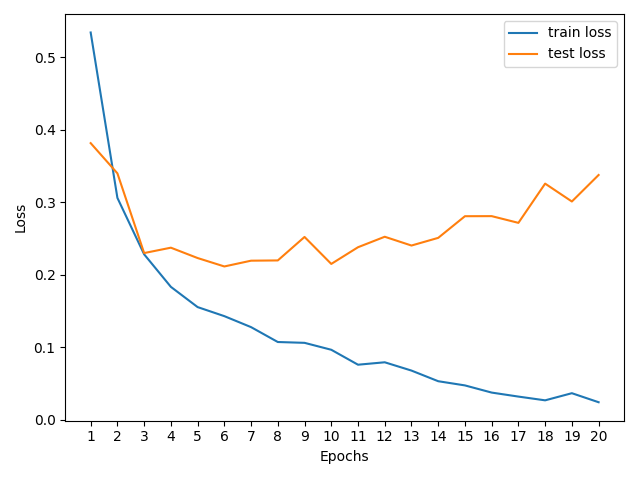
\includegraphics[width=0.4\textwidth]{a1_learning_curve.png}
    		\caption{The learning curve for the training of the CNN implemented to solve task A1. As can be seen, the testing error has a minimum point. For epochs greater than 8, the loss increases slowly suggesting an over-fit model as the training accuracy continues to decrease.}
    		\label{fig:a1_leraning_curve}
    	\end{figure}
    
    	The neural network was created by utilizing the {\tt keras} and {\tt tensorflow} packages. In order to achieve maximum flexibility with the model a custom model was created by sub-classing from {\tt keras.models.Model}. All layers used in this model are provided by {\tt keras} and their parameters were tuned by using k-fold CV. Initially, the model was compiled using the Adam optimizer and the sparse categorical cross entropy loss function. Following this, the model was trained on the training dataset. By subclassing from {\tt keras.models.Model}, it was possible to obtain intermediate outputs of the max pooling layers to visualize the effect of the filters. The images in Appendix \ref{sec:a1_cnn_filter_outputs} show the outputs of the first and second set of filters (the outputs of the MAXPOOL layers in Fig. \ref{fig:a1_cnn}) respectively. 
    	\\
    	
    	The {\tt keras} module trains on the dataset in epochs. The number of epochs is user-defined and defines when the learning will cease. The optimal number of epochs were chosen as 7 from the learning curve shown in Fig. \ref{fig:a1_leraning_curve}.
    	\\
    	
    	As {\tt keras} does not have a built in function for cross-validation and hyper-parameter tuning, a custom function was utilized. This function iterates through all combinations of hyper-parameters defined by the user and computes the average accuracy over k folds of the training dataset. To obtain the k split dataset the {\tt StratifiedKFold} class from {\tt sklearn} was utilized. This chooses k subsets of the training dataset each of which are representative in their class distribution to the whole training set. In addition to tracking accuracy, training time, pre-processing time are also tracked and used to make a final decision on the optimal hyper-parameters shown in Fig. \ref{fig:a1_cnn}.
    	
    \subsection{Task A2: Emotion Classification (Binary)}
 	\label{sec:implement_A2}
 	
 		Task A2 is to classify the emotion of the person in the image using the labels smiling and not smiling. Therefore it would be beneficial to extract features from the mouth portion of the face. For detection of facial features, the face was read into memory in greyscale format. Initially, an attempt was made to use pre-trained haar cascade classifiers from the {\tt OpenCV} modules to detect mouths in the face image. However, this was unsuccessful as the classifier would detect multiple mouths or detect none at all in too many cases. When detecting the faces using the haar cascade classifier, the proportion of faces identified were less than 60\% and therefore insufficient in accuracy to be used. As an alternate approach, the faces were detected using a classic History of Oriented Gradients (HOG) feature combined with a linear classifier, an image pyramid and sliding window detection scheme. An implementation of this approach in the {\tt dlib} module was used. This method was able detect more than 95\% of the faces in the images. The images fed into the face detector were greyscale versions of the original images without any scaling.
 		\\
 		
 		Following the face detection, landmarks were extracted from the detected face using an Ensemble of Regression Trees \autocite{6909637}. This too was implemented in {\tt dlib} with a downloadable pre-trained model. Any faces that weren't detected were discarded from the training process, however during the testing process all samples receive a predicted label. The total number of landmarks extracted were 68 and an example of all the landmarks are shown in \ref{fig:68_landmarks_all}. As we are only concerned with the mouth of the subject, landmarks 48 to 68 were extracted and used as features to train the model.
 		\\
 		
 		\begin{figure}[htb]
 			\centering
 			\begin{subfigure}{0.2\textwidth}
 				\centering
 				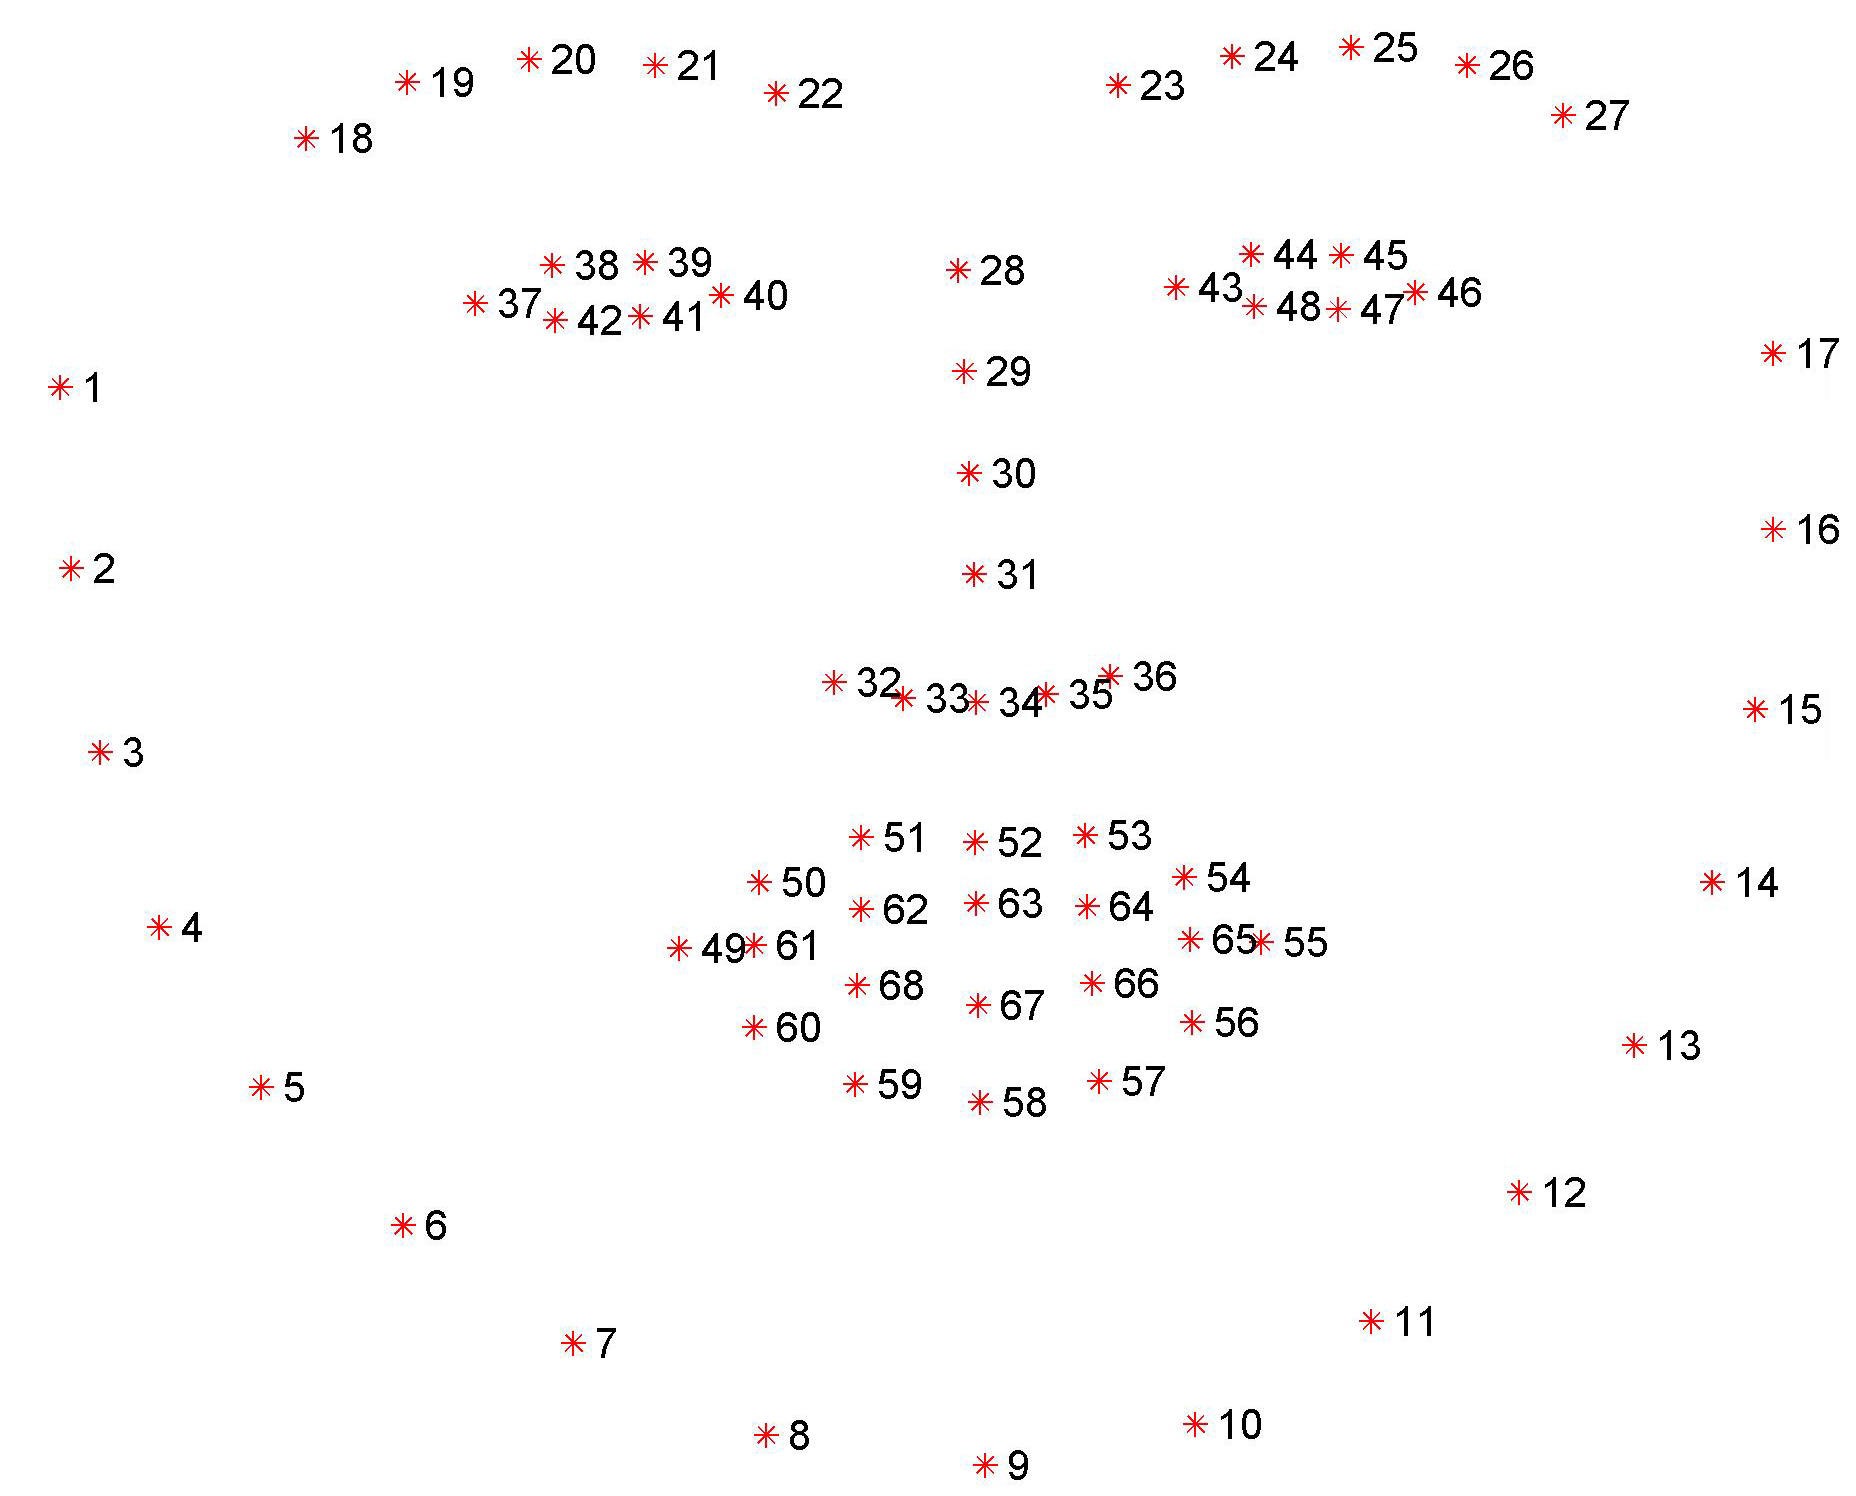
\includegraphics[scale=0.05]{68_landmarks.jpg}
 				\caption{The 68 facial landmarks labelled taken from the dataset used to train the classifier that was used \autocite{ibug_dataset}}
 				\label{fig:68_landmarks}	
 			\end{subfigure}
 			\hspace{1em}
 			\begin{subfigure}{0.2\textwidth}
 				\centering
 				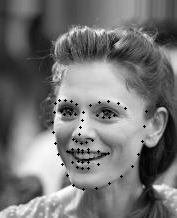
\includegraphics[scale=0.5]{68_landmark_sample.png}
 				\caption{A sample image with the landmarks labelled as black dots.}
 				\label{fig:68_landmark_sample}	
 			\end{subfigure}
 			\caption{images depicting the 68 extracted facial landmarks.}
 			\label{fig:68_landmarks_all}
 		\end{figure}
 		
 		Using these landmarks, initially an attempt was made to reduce the features down to a single feature. An aspect ratio of the mouth was computed similar to the approach discussed in \autocite{soukupova2016}. The formula discussed in \autocite{8751886} to compute the mouth aspect ratio (MAR) was used as a feature to classify the smile. However this yielded accuracies close to 50\% suggesting that the model was as good as guessing and was hence abandoned. 
 		\\
 		
 		\begin{figure}[htb]
 			\centering
 			\begin{subfigure}{0.2\textwidth}
 				\centering
 				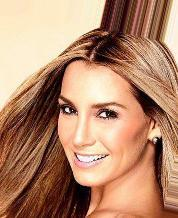
\includegraphics[width=0.8\textwidth]{a2_original_img.jpg}
 				\caption{The original image in colour.}
 				\label{fig:a2_original_img}	
 			\end{subfigure}
 			\hspace{1em}
 			\begin{subfigure}{0.2\textwidth}
 				\centering
 				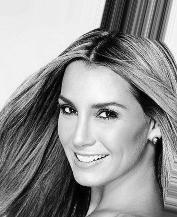
\includegraphics[width=0.8\textwidth]{a2_greyscale_img.png}
 				\caption{Image converted to greyscale for easier processing}
 				\label{fig:a2_greyscale_img}	
 			\end{subfigure}
 			\\
 			\begin{subfigure}{0.2\textwidth}
 				\centering
 				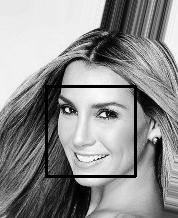
\includegraphics[width=0.8\textwidth]{a2_face_bb.png}
 				\caption{Bounding box around the detected face}
 				\label{fig:a2_face_bb}	
 			\end{subfigure}
 			\hspace{1em}
 			\begin{subfigure}{0.2\textwidth}
 				\centering
 				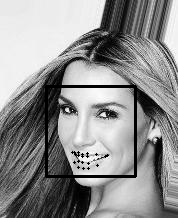
\includegraphics[width=0.8\textwidth]{a2_mouth_landmarks.png}
 				\caption{The 21 of the 68 detected landmarks on the face}
 				\label{fig:a2_mouth_landmarks}	
 			\end{subfigure}
 			\caption{A visual representation of the feature extraction for this task.}
 			\label{fig:a2_pre_processing}
 		\end{figure}
 		
 		The chosen approach was to use the mouth landmarks as features to train the model. However, prior to passing them as inputs, the coordinates were normalized. This was done by subtracting the mean x and y coordinates from the x and y coordinates of each of the landmarks. Having done this, the values are then scaled to have a maximum magnitude of 1 (i.e in the range $[-1, 1]$). This normalization ensures that the mouths are of similar shape, and the model doesn't prioritize larger mouths to smaller ones. Having normalized the coordinates, these coordinates are then used as features for the model to train on. The different stages of the pre-processing of the image are presented for one image sample in Fig. \ref{fig:a2_pre_processing}.
 		\\
 		
 		Following the extraction and normalization of the mouth landmarks, the SVM model implementation in {\tt sklearn} was utilized as the model for this task. This implementation has quick access to change parameters such as the kernel, regularization parameter and kernel parameters such as polynomial degree. In addition to this, by choosing a classifier from the {\tt sklearn} module, access to hyper-parameter tuning tools such as {\tt GridSearchCV}. This tool was utilized to tune the hyper-parameters of the SVM model. The final chosen parameters are a polynomial kernel with a degree of 5 and a regularization parameter (C) of 100. 
 		\\
 		
 		\begin{figure}[htb]
 			\centering
 			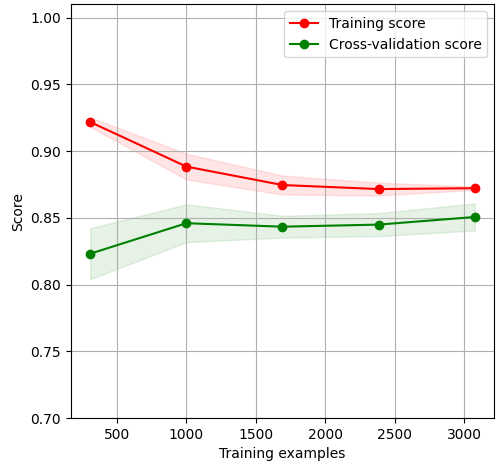
\includegraphics[width=0.4\textwidth]{a2_learning_curve.png}
 			\caption{The learning curve for the training of the SVM for task A2 on increasing number of samples. On a small dataset the SVM over-fits. With increasing number of samples the training and validation accuracy converge to the same value.}
 			\label{fig:a2_leraning_curve}
 		\end{figure}
 		
 		SVMs have no stopping criterion as the training it not iterative, however the convergence of the model can be viewed by observing the SVM accuracy convergence for increasing sample sizes as shown in Fig. \ref{fig:a2_leraning_curve}. The SVM over-fits at small sample sizes which is conveyed by the large difference in the training accuracy and validation accuracy. However, with increasing sample sizes, the model training and validation accuracy converge to the same value resulting in convergence to a solution.
 		
    \subsection{Task B1: Face-Shape Classification (Multi-Class)}
    \label{sec:implement_B1}
	    
	    For this task, the symmetrical nature of the images in the dataset was exploited by utilizing only half of the image for classification. As the colours in the image aren't essential to classifying the face-shape of the cartoon, the image was read into memory as a greyscale image using the {\tt OpenCV} module. Following this, the image was cropped to half it's size; This means that an image that was originally 500x500 will be cropped to an image of size 250x500. Furthermore, the images are downscaled to 25x50. Finally, the individual pixel values are normalized similar to the approach for task A1 described in \S \ref{sec:implement_A1}. 
	    \\
	    
	    The model used to classify the processed images is once again an SVM and the implementation as well as tuning of the model is identical to the approach described in \S \ref{sec:implement_A2}. The {\tt SVC} class from the {\tt sklearn} module was utilized for the implementation of the SVM and {\tt GridSearchCV} was utilized for hyper-parameter tuning. To minimize the time taken for the model to train and make predictions a linear kernel with a regularization parameter (C) of 1 was chosen. 
	    \\
	    
	    \begin{figure}[htb]
	    	\centering
	    	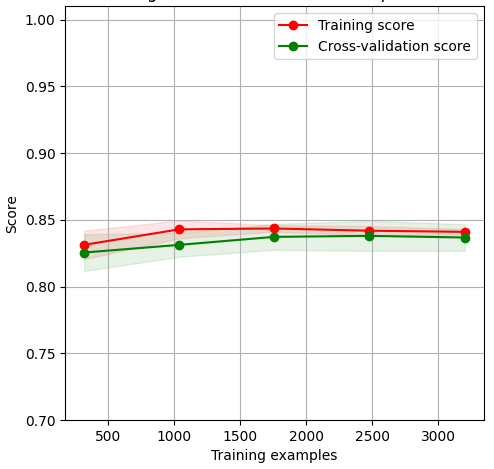
\includegraphics[width=0.4\textwidth]{b1_learning_curve.png}
	    	\caption{The learning curve for the training of the SVM for task B1 on increasing number of samples.}
	    	\label{fig:b1_leraning_curve}
	    \end{figure}
	    
	    The learning curve for the training of the SVM in this scenario suggests that the model was able to converge to a solution much quicker. So much so that the convergence itself is not visible in Fig. \ref{fig:b1_leraning_curve}, instead both the training accuracy and the validation accuracy track a constant accuracy score.
	    
    \subsection{Task B2: Eye-Colour Classification (Multi-Class)}
    \label{sec:implement_B2}
	    
	    For this task a similar approach to that in task B1 was taken. The symmetry of the faces was exploited once again by cropping the faces to half their original size. This time however, the colours in the image carry important information for the class labels and therefore, the image was read into memory in full colour using {\tt OpenCV}. The images were then resized from 250x500 to 20x40. This dimension was chosen to minimize the number of features while still achieving reasonable accuracy results. Finally, the pixel values are normalized in an identical fashion to the way it was previously discussed in \ref{sec:implement_A1}. As the images have a lot of white pixels that do not change from one image to the next, a low variance filter was fitted on the training dataset with a threshold of 0.16. This corresponds to any features that are identical for all of the dataset being fitted. Once fitted on the training dataset, the same filter is also applied to the testing dataset and any future inputs to the model. This low variance removes any features that are identical for all of the dataset, thereby reducing the dimensionality of the data. The mask for this filter can be seen in Fig. \ref{fig:lv_mask}.
	    \\
	    
	    \begin{figure}[htb]
	    	\centering
	    	
\includegraphics[width=0.2\textwidth]{lv_mask.png}
	    	\caption{The mask fitted by the low variance filter. The area in black marks pixels that were discarded due to no variation amongst the dataset. The actual mask is half of this due to the cropping of the image but for interpretation sake, it was reflected.}
	    	\label{fig:lv_mask}
	    \end{figure}
	    
	    The model used for this problem is a random forest and when realising the model, the \texttt{RandomForestClassifier} class from \texttt{sklearn} was used. Once again when tuning hyper-parameters the \texttt{GridSearchCV} class from \texttt{sklearn} was utilized. The most optimal parameters in terms of execution time and accuracy were 100 decision trees with a splitting criterion of gini. The maximum depth of each decision tree was limited to 5.
	    \\
	    
	    \begin{figure}[htb]
	    	\centering
	    	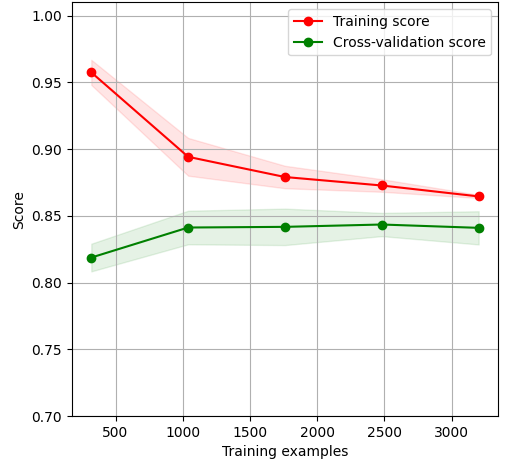
\includegraphics[width=0.4\textwidth]{b2_learning_curve.png}
	    	\caption{The learning curve for the training of the random forest for task B2 on increasing number of samples.}
	    	\label{fig:b2_leraning_curve}
	    \end{figure}
	    
	    Similar to Task A2 as described at the end of \S \ref{sec:implement_A2}, the model initially over-fits due to the small sample size. But with incresing samples, the model is able to converge its training accuracy. Both the training score and the validation score seem to be converging to the same score.

\section{Experimental Results and Analysis}
\label{sec:experimental_results}

	\begin{table}[H]
		\centering
		\label{table:Table1}
		\begin{tabular}{@{}lllll@{}}
			\toprule
			Task & Model & Train Acc & Val Acc & Test Acc \\ \midrule
			A1   & CNN   & 95.3\%    & 92.2\%  & 91.1\%   \\
			A2   & SVM   & 87.5\%    & 85.2\%  & 84.5\%   \\
			B1   & SVM   & 99.5\%    & 98.3\%  & 99.0\%   \\
			B2   & RF    & 83.6\%    & 82.7\%  & 83.0\%   \\ \bottomrule
		\end{tabular}
	\end{table}
    
    Having, trained and hyper-parameter tuned all models, the models were finally tested on a completely unseen test dataset. This dataset had never been trained on in any way. The results in the table above depict all the results. The "Train Acc" is the accuracy of the model on the training data and the "Val Acc" is the k-fold validation average accuracy of the best hyper-parameter combination. Finally, the "Test Acc" is the accuracy of the model on the unseen testing dataset. Overall, the learnt models performed well having a small deviation between the training accuracy and testing accuracy.
    \\
    
    As can be seen from the table, for task A1, the CNN model that was implemented was able to achieve an accuracy of 91.1\% on the unseen test dataset. As the training accuracy is at 95.3\% this may suggest a slight degree of over-fitting. This could potentially have been avoided by the utilization of dropout layers in the CNN. For task A2 the major limiting factor in the accuracy was most likely the fact that a proportion of the faces were not detected by the face detector. In such a case, all features are set to zero resulting in all undetected faces having the same predicted class. The main cases of faces that weren't detected are those where the face is viewed side on. Task B1 was able to converge well to a solution and shows minimal signs of over-fitting as it performed exceptionally well on the test set with an accuracy of 99.0\%. Finally, task B2 shows relatively bad results with a test accuracy of 83.0\%. However, it should be noted that around 10\% of the characters in the dataset had obstacles blocking the eyes making it impossible in these cases to predict the eye-colour. This is also reflected in the larger number of erroneous black eye predictions shown in the confusion matrix in Appendix \ref{fig:confusion matrices}.
    

\section{Conclusion}
\label{sec:conclusion}
    From the results obtained and presented in \S \ref{sec:experimental_results}, it is clear to see that the machine learning models perform reasonably well. Then CNN performed well as expected with classifying the gender of the human face images. It was able to extract features from the faces and the resulting output of the filters is shown in Appendix \ref{sec:a1_cnn_filter_outputs}. A more robust facial detection classifier would have resulted in the model for A2 being more performant. For tasks B1 and B2 the models performed as well as they could have. One of the remarks that could be made is that during training, the samples that have obstructed eyes should be discarded from the training process to prevent these outliers from influencing the model. Additionally, it is evident that the cartoonset dataset has very little noise meaning that the models are very likely to have been over-fit to the dataset. 

% References should be produced using the bibtex program from suitable
% BiBTeX files (here: strings, refs, manuals). The IEEEbib.bst bibliography
% style file from IEEE produces unsorted bibliography list.
% -------------------------------------------------------------------------
\printbibliography

\clearpage
\onecolumn
\appendix
\appendixpage

\section{Filter Outputs of CNN for Task A1}
\label{sec:a1_cnn_filter_outputs}

	\begin{figure}[H]
		\centering
		\begin{subfigure}{0.75\textwidth}
			\centering
			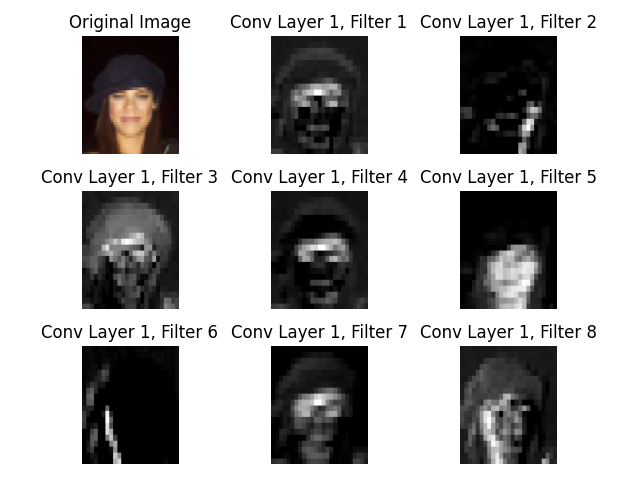
\includegraphics[width=0.8\textwidth]{cnn_filter1.png}
			\caption{The outputs of the first set of convolutional and max pooling layers. The original image is also shown for reference.}
			\label{fig:cnn_filter1}	
		\end{subfigure}
		\begin{subfigure}{0.75\textwidth}
			\centering
			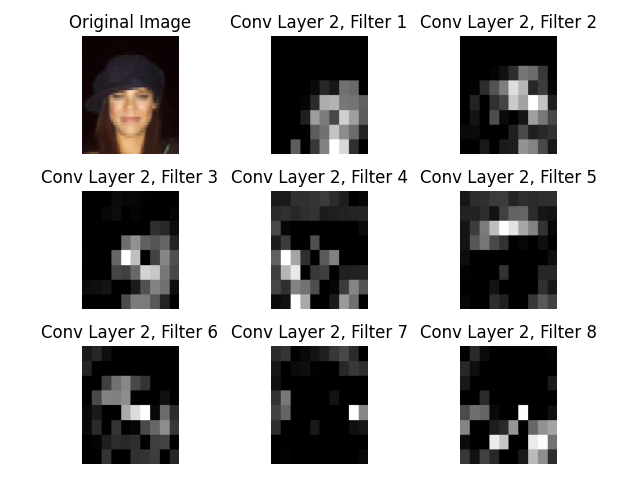
\includegraphics[width=0.8\textwidth]{cnn_filter2.png}
			\caption{The outputs of the second set of convolutional and max pooling layers. The original image is also shown for reference.}
			\label{fig:cnn_filter2}	
		\end{subfigure}
		\caption{The plots depicting the outputs of the two convolutional layers implemented for a sample test input}
		\label{fig:cnn_filter_output}
	\end{figure}

\clearpage
\section{Confusion Matrices for all Tasks}
\label{sec:confusion_matrices}

	\begin{figure}[H]
		\begin{subfigure}{0.5\textwidth}
			\centering
			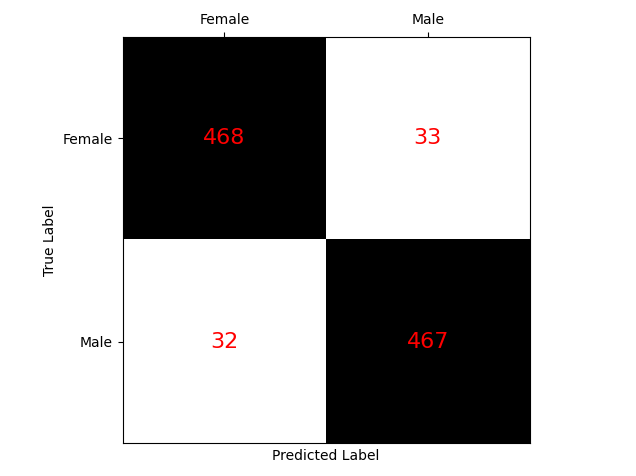
\includegraphics[width=0.8\textwidth]{a1_confusion_matrix.png}
			\caption{Confusion matrix for task A1.}
			\label{fig:a1_confusion_matrix}	
		\end{subfigure}
		\begin{subfigure}{0.5\textwidth}
			\centering
			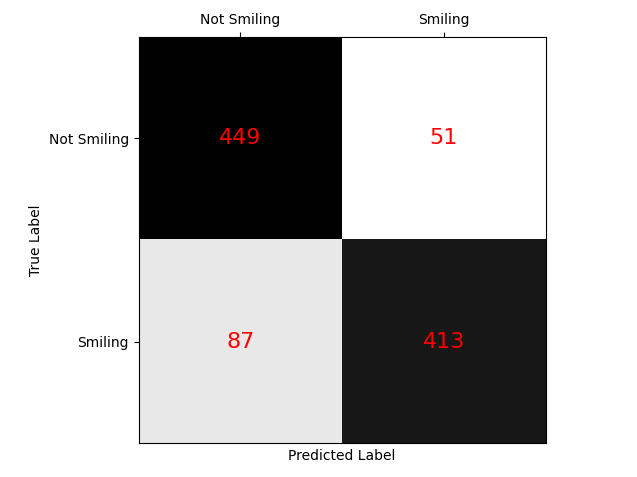
\includegraphics[width=0.8\textwidth]{a2_confusion_matrix.png}
			\caption{Confusion matrix for task A2.}
			\label{fig:a2_confusion_matrix}	
		\end{subfigure}
		\begin{subfigure}{0.5\textwidth}
			\centering
			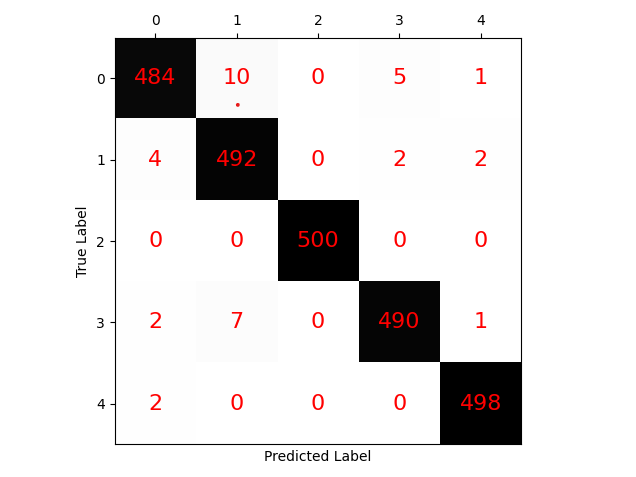
\includegraphics[width=0.8\textwidth]{b1_confusion_matrix.png}
			\caption{Confusion matrix for task B1.}
			\label{fig:b1_confusion_matrix}	
		\end{subfigure}
		\begin{subfigure}{0.5\textwidth}
			\centering
			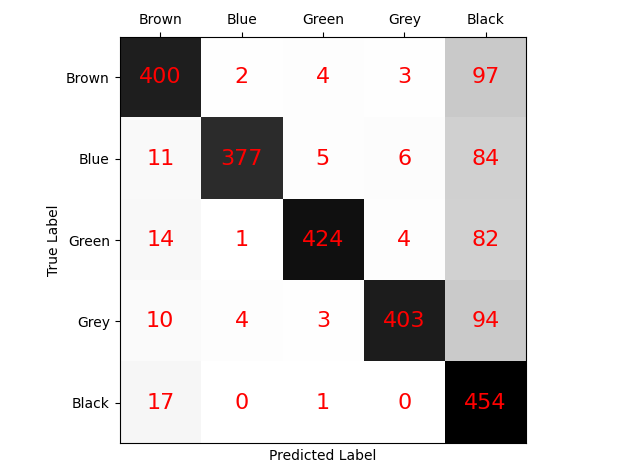
\includegraphics[width=0.8\textwidth]{b2_confusion_matrix.png}
			\caption{Confusion matrix for task B2.}
			\label{fig:b2_confusion_matrix}	
		\end{subfigure}
		\caption{Confusion matrices for the predictions on the unseen test dataset}
		\label{fig:confusion matrices}
	\end{figure}
	

\end{document}
